%%%%%%%%%%%%%%%%%%%%%%%%%%%%%%%%%%%%%%%%%
% Simple Sectioned Essay Template
% LaTeX Template
%
% This template has been downloaded from:
% http://www.latextemplates.com
%
% Note:
% The \lipsum[#] commands throughout this template generate dummy text
% to fill the template out. These commands should all be removed when 
% writing essay content.
%
%%%%%%%%%%%%%%%%%%%%%%%%%%%%%%%%%%%%%%%%%

%----------------------------------------------------------------------------------------
%	PACKAGES AND OTHER DOCUMENT CONFIGURATIONS
%----------------------------------------------------------------------------------------

%\documentclass[12pt]{article} % Default font size is 12pt, it can be changed here

%\usepackage{geometry} % Required to change the page size to A4
%\geometry{letterpaper} % Set the page size to be A4 as opposed to the default US Letter

%\usepackage{graphicx} % Required for including pictures

%\usepackage{listings} %Para comandos bash Linux

%\usepackage{float} % Allows putting an [H] in \begin{figure} to specify the exact location of the figure
%\usepackage{wrapfig} % Allows in-line images such as the example fish picture

%\usepackage{color} %textos de colores

%\usepackage[spanish]{babel}

%\usepackage[utf8]{inputenc} %Uso de acentos directamente

%\usepackage{hyperref}

%\linespread{1.2} % Line spacing

%\setlength\parindent{0pt} % Uncomment to remove all indentation from paragraphsre

%\graphicspath{{Pictures/}} % Specifies the directory where pictures are stored

%\begin{document}

%----------------------------------------------------------------------------------------
%	TITLE PAGE
%----------------------------------------------------------------------------------------

%\begin{titlepage}

%\newcommand{\HRule}{\rule{\linewidth}{0.5mm}} % Defines a new command for the horizontal lines, change thickness here

%\center % Center everything on the page

%\textsc{\LARGE Universidad Autónoma de Yucatán}\\[1.5cm] % Name of your university/college
%\textsc{\Large Facultad de Matemáticas}\\[0.5cm] % Major heading such as course name
%\textsc{\large Anexo de tesis de Alex Antonio Turriza Suárez}\\[0.5cm] % Minor heading such as course title

%\HRule \\[0.4cm]
%{ \huge \bfseries Configuración de un Sistema de Archivos en Red [NFS] entre una PC x86-64 y una BeagleBone Black}\\[0.4cm] % Title of your document
%\HRule \\[1.5cm]
%\begin{minipage}{0.5\textwidth}
%\begin{flushleft} \large
%\emph{Autor:}\\
%Alex Antonio \textsc{Turriza Suárez} % Your name
%\end{flushleft}
%\end{minipage}
%~
%\begin{minipage}{0.4\textwidth}
%\begin{flushright} \large
%\emph{Asesores:} \\
%Dr. Arturo \textsc{Espinosa Romero} \\
%\ \ \\
%Dr. Anabel \textsc{Martín González}
%\end{flushright}
%\end{minipage}\\[4cm]

%{\large \today}\\[3cm] % Date, change the \today to a set date if you want to be precise

%\includegraphics{Logo}\\[1cm] % Include a department/university logo - this will require the graphicx package

%\vfill % Fill the rest of the page with whitespace

%\end{titlepage}

%----------------------------------------------------------------------------------------
%	TABLE OF CONTENTS
%----------------------------------------------------------------------------------------

%\tableofcontents % Include a table of contents

%\newpage % Begins the essay on a new page instead of on the same page as the table of contents 

%----------------------------------------------------------------------------------------
%	INTRODUCTION
%----------------------------------------------------------------------------------------
\chapter{Sistema de Archivos en Red entre una PC y una BeagleBone Black}\label{Anx:nfs}
\section{Introducción}
Cuando dos máquinas de diferente arquitectura deben trabajar en un sólo proyecto, suele suceder que es mucho más cómodo realizar código y documentación en una, a pesar de que que los archivos estén destinados a ser usados en la otra.

Para ello, se mostrará la forma de configurar un sistema de archivos en red NFS que facilite la tarea de compartir archivos en un directorio.

En este trabajo se mostrará la instalación del sistema en una máquina host en una PC y un cliente en una BeagleBone Black, aprovechando que al conectar mediante USB, se crea una red entre ambas plataformas.

%------------------------------------------------

\section{Definición de NFS}
Sistema de archivos en red (NFS, "\textit{Network File System}" por sus siglas en inglés), es un protocolo que permite acceder mediante una conexión remota a un sistema de archivos [\href{https://debian-handbook.info/browse/es-ES/stable/sect.nfs-file-server.html}{El Manual del Administrador de Debian}\footnotemark, consultado en Octubre 2016].

\footnotetext{\href{https://debian-handbook.info/browse/es-ES/stable/sect.nfs-file-server.html}{https://debian-handbook.info/browse/es-ES/stable/sect.nfs-file-server.html}}

En su funcionamiento, permite que un equipo host comparta determinado directorio con otros equipos clientes, pudiendo determinar qué equipos tienen permisos de lectura, escritura o ambas.

%------------------------------------------------

\section{Descarga e instalación}\label{sec:_install} % Sub-section

\subsection{Instalación en host / PC}
Bajo Ubuntu en sus últimas versiones en el momento de la redacción de éste documento, se abre una terminal con los comandos \textit{Ctrl + Alt + t}.

Lo primero, es actualizar los repositorios con:
\begin{lstlisting}[language=bash]
$ sudo apt-get update
\end{lstlisting}

Una vez actualizados, se procede a la instalación de un paquete mediante el siguiente comando:

\begin{lstlisting}[language=bash]
$ sudo apt-get install nfs-kernel-server 
\end{lstlisting}

Al finalizar la descarga e instalación, se debe modificar un archivo. Copiar en la terminal el siguiente comando y colocar la contraseña:
\begin{lstlisting}[language=bash]
$ sudo nano /etc/default/nfs-kernel-server
\end{lstlisting}

Se debe modificar la línea \textbf{NEED\_SVCGSSD=""} y colocar $"no"$ en el entrecomillado, como muestra la figura \ref{fig:NFSKer}. Cuando se termine de modificar, guardar con la combinación de teclas $Ctrl + O$ y regresar a la terminal con $Ctrl + X$.

\begin{figure}[H] % Example image
\center{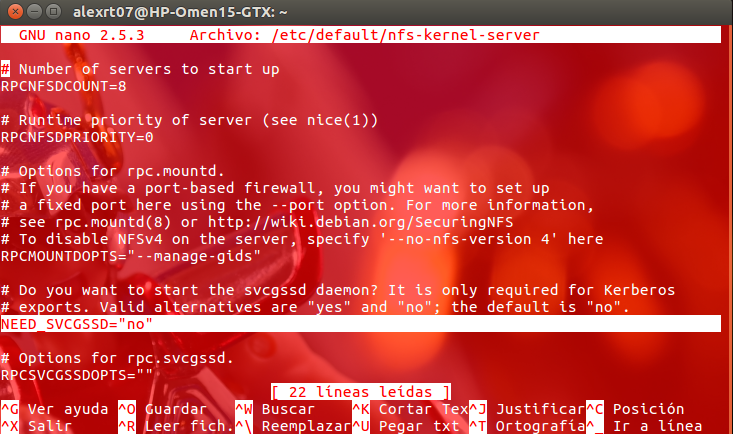
\includegraphics[width=0.9\linewidth]{Figures/NFS/NFS1}}
\caption{Archivo /etc/default/nfs-kernel-server ya modificado.}
\label{fig:NFSKer}
\end{figure}

Lo siguiente es abrir el archivo ubicado en /etc/idmapd.conf:
\begin{lstlisting}[language=bash]
$ sudo nano /etc/idmapd.conf 
\end{lstlisting}

Verificar que existan las líneas $Nobody-User = nobody$ y $Nobody-Group = nogroup$ como muestra la figura \ref{fig:NFSKer2}.

\begin{figure}[H] % Example image
\center{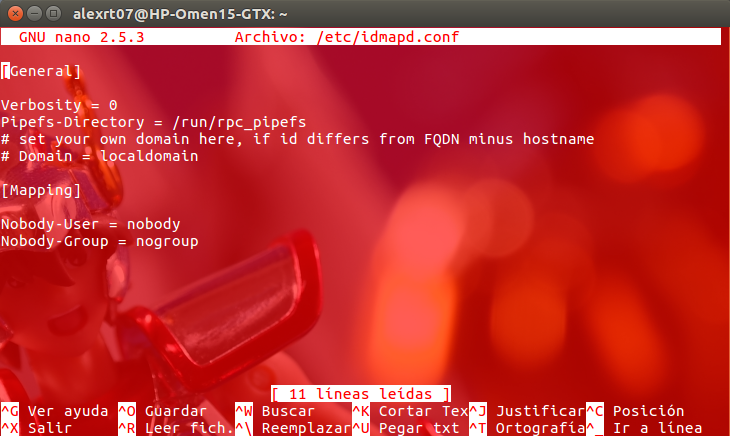
\includegraphics[width=0.9\linewidth]{Figures/NFS/NFS2}}
\caption{Archivo /etc/idmapd.conf.}
\label{fig:NFSKer2}
\end{figure}

Cuando se realiza una conexión con la BeagleBone Black mediante un cable USB, se crea una red con las siguientes direcciones: $192.168.7.2$ para la BeagleBone y $192.168.7.1$ para el PC host. Entonces, tomando en cuenta lo anterior, se modifica el archivo /etc/exports de la siguiente manera:

Se abre el archivo con nano, en la terminal:

\begin{lstlisting}[language=bash]
$ sudo nano /etc/exports
\end{lstlisting}

En el archivo que se abre, añadir la siguiente línea (note que dentro del paréntesis, entre los comandos no existen espacios):

\begin{lstlisting}[language=bash]
/home/alexrt07/Escritorio/Alex     192.168.7.2(rw,sync,
no_root_squash,no_subtree_check)
\end{lstlisting}

Donde /home/alexrt07/Escritorio/Alex es el directorio a compartir y 192.168.7.2 es la dirección ip de la BeagleBone. Así, el archivo queda como muestra la figura \ref{fig:NFSKer3}.

\begin{figure}[H] % Example image
\center{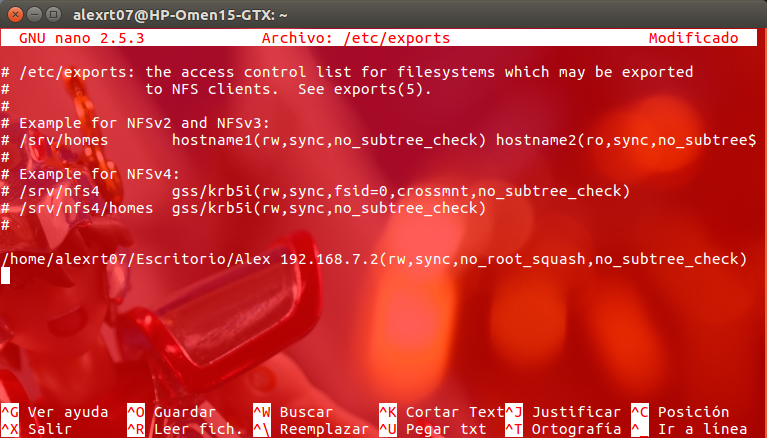
\includegraphics[width=0.9\linewidth]{Figures/NFS/NFS3}}
\caption{Archivo /etc/exports.}
\label{fig:NFSKer3}
\end{figure}

Finalmente, resta reiniciar el servidor con el siguiente comando: 

\begin{lstlisting}[language=bash]
$ /etc/init.d/nfs-kernel-server restart
\end{lstlisting}

Se deberá mostrar una confirmación de reinicio exitoso.
%---------------------------------------------------

\subsubsection{Seguridad}\label{subsec:conf}

Para evitar dejar hoyos de seguridad de acceso a los archivos personales, es altamente recomendable modificar los archivos /etc/hosts.deny y /etc/hosts.allow para permitir acceso solamente a los clientes conocidos.

Abrir el archivo /etc/hosts.deny con:

\begin{lstlisting}[language=bash]
$ sudo nano /etc/hosts.deny
\end{lstlisting}

Y añadir la siguiente línea:

\begin{lstlisting}[language=bash]
rpcbind mountd nfsd statd lockd rquotad : ALL
\end{lstlisting}

\begin{figure}[H] % Example image
\center{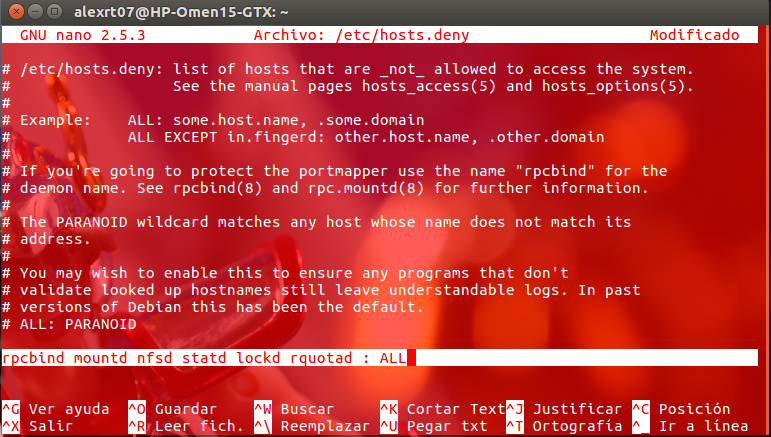
\includegraphics[width=0.9\linewidth]{Figures/NFS/NFS4}}
\caption{Archivo /etc/hosts.deny}
\label{fig:NFSKer4}
\end{figure}

Como muestra la figura \ref{fig:NFSKer4}. Ahora, abrir el archivo /etc/hosts.allow con el comando:

\begin{lstlisting}[language=bash]
$ sudo nano /etc/hosts.allow
\end{lstlisting}

Y añadir la siguiente línea:

\begin{lstlisting}[language=bash]
  rpcbind mountd nfsd statd lockd 
  rquotad : 192.168.7.2 127.0.0.1 
\end{lstlisting}

Como muestra la figura \ref{fig:NFSKer5}.

\begin{figure}[H] % Example image
\center{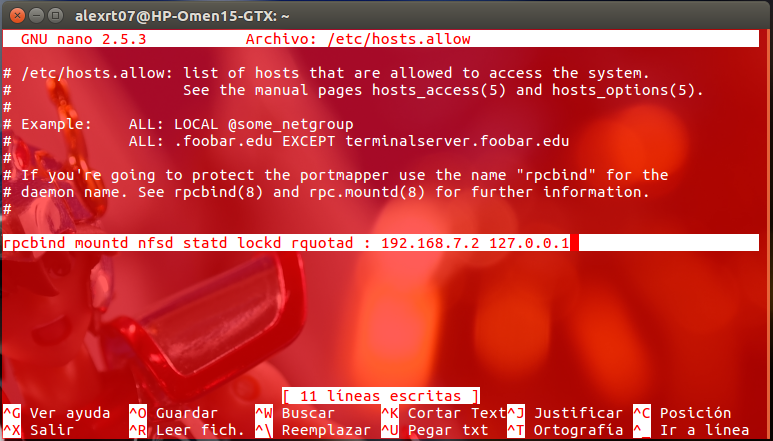
\includegraphics[width=0.9\linewidth]{Figures/NFS/NFS5}}
\caption{Archivo /etc/hosts.allow}
\label{fig:NFSKer5}
\end{figure}

Reiniciar el servidor con: 

\begin{lstlisting}[language=bash]
$ service nfs-kernel-server restart
\end{lstlisting}

Ahora, el PC está preparado para compartir vía red el directorio:

\begin{lstlisting}[language=bash]
/home/alexrt07/Escritorio/Alex/
\end{lstlisting}

\subsection{Instalación en cliente / BeagleBone}

Asumiendo que la BeagleBone Black tiene un Debian con su archivo \textit{/etc/apt/sources.list} correctamente configurado, ejecutamos en la terminal de nuestro host para conectarnos:

\begin{lstlisting}[language=bash]
$ ssh -l root 192.168.7.2
\end{lstlisting}

donde \textit{ssh} es el comando para conectarse por el protocolo secure shell, \textit{-l} es el comando que indica que se hará un login con el usuario \textit{root}, y \textit{192.168.7.2} es la dirección IP de la BeagleBone en la red que se creó a través del cable USB.

Entonces, una vez hecho el loggin, ejecutar:

\begin{lstlisting}[language=bash]
$ apt-get install nfs-common
\end{lstlisting}

Que instalará y preconfigurará los archivos necesarios para una correcta comunicación a través de NFS.

Es recomendable crear un directorio en donde se montarán los archivos que compartirá con la PC:

\begin{lstlisting}[language=bash]
$ mkdir /home/debian/Alex_tesista
\end{lstlisting}

\section{Ejecución}

Se procede a montar el sistema de archivos con el siguiente comando:

\begin{lstlisting}[language=bash]
$ mount -t nfs -o proto=tcp,port=2049 
  192.168.7.1:/home/alexrt07/ARM-Root/home/Alex 
  /home/debian/Alex_tesista/
\end{lstlisting}

En donde \textit{mount} es el comando para montar el directorio, \textit{-t nfs} indica que se trata de un sistema de archivos por red, \textit{-o proto=tcp,port=2049} indica que se utilizará el protocolo de transferencia de archivos a través del puerto 2049 (mirar el manual de nfs en su página 5 con \textbf{\$ man 5 nfs} para más opciones e información),\textit{192.168.7.1:} es la dirección IP de la PC host, \textit{/home/alexrt07/ARM-Root/home/Alex} es el directorio que contiene los archivos a compartir, y \textit{/home/debian/Alex\_tesista/} es el directorio creado en donde se encontrarán los archivos.

Para cerrar esta conexión, utilice

\begin{lstlisting}[language=bash]
$ umount /home/debian/Alex_tesista/
\end{lstlisting}

Tome en cuenta que al finalizar la conexión, no se mantendrán los archivos compartidos por nfs. Desaparecerán y contendrá los archivos originales que esa carpeta contenía antes de montar el sistema de archivos por red.

%\end{document}